\documentclass[11pt,a4paper]{article}

\usepackage[T1]{fontenc}
\usepackage[utf8]{inputenc}
\usepackage{lmodern}
\usepackage{microtype}
\usepackage[a4paper,margin=25mm,headheight=14pt]{geometry}
\usepackage{amsmath,amssymb}
\usepackage{booktabs}
\usepackage{graphicx}
\usepackage{caption}
\usepackage{float}
\usepackage{enumitem}
\usepackage{fancyhdr}
\usepackage[round,authoryear]{natbib}
\usepackage[hidelinks]{hyperref}

\hypersetup{
  pdftitle={Signed order count in aggregate price impact: TSLA, 2019},
  pdfauthor={Riad Darwish},
  pdfsubject={Empirical market microstructure study using LOBSTER event data},
  pdfkeywords={market impact, order flow imbalance, market microstructure, LOBSTER, TSLA}
}

% Values reported in the tables and text. Sources: aggregate files under ../results/.
\newcommand{\DeliveredSessions}{252}
\newcommand{\Sessions}{249}
\newcommand{\CoverageExcludedSessions}{3}
\newcommand{\MaximumCoverageGapSeconds}{60}
\newcommand{\VisibleOrders}{4{,}547{,}078}
\newcommand{\ScalingTransactions}{5{,}845{,}437}
\newcommand{\MedianDailyOrders}{16{,}049}
\newcommand{\PtenDailyOrders}{10{,}839}
\newcommand{\PninetyDailyOrders}{29{,}935}
\newcommand{\MedianOrderSize}{55}
\newcommand{\PninetyOrderSize}{195}
\newcommand{\PninetynineOrderSize}{700}
\newcommand{\MedianSpread}{7.0}
\newcommand{\PninetySpread}{15.0}
\newcommand{\BuyerFraction}{49.7\%}
\newcommand{\TenOrderWindows}{454{,}576}
\newcommand{\TenOrderImpactSd}{12.46}
\newcommand{\ZeroImpactFraction}{3.0\%}
\newcommand{\TrainFirstDate}{2019-01-02}
\newcommand{\TrainLastDate}{2019-10-17}
\newcommand{\TestFirstDate}{2019-10-18}
\newcommand{\TestLastDate}{2019-12-31}
\newcommand{\TrainObservations}{352{,}108}
\newcommand{\TestObservations}{102{,}468}
\newcommand{\BaselineRtwo}{0.118}
\newcommand{\VolumeRtwo}{0.298}
\newcommand{\RawCountRtwo}{0.359}
\newcommand{\AugmentedRtwo}{0.360}
\newcommand{\VolumeMse}{117.16}
\newcommand{\RawCountMse}{106.93}
\newcommand{\DeltaRtwo}{0.061}
\newcommand{\MseReduction}{8.7\%}
\newcommand{\TotalMseReduction}{27.4\%}
\newcommand{\BootstrapDeltaLower}{0.056}
\newcommand{\BootstrapDeltaUpper}{0.066}
\newcommand{\BootstrapMseLower}{8.0\%}
\newcommand{\BootstrapMseUpper}{9.5\%}
\newcommand{\BootstrapClusters}{51}
\newcommand{\BootstrapReplicates}{10{,}000}
\newcommand{\TrimmedBaselineRtwo}{0.241}
\newcommand{\TrimmedAugmentedRtwo}{0.383}
\newcommand{\TrimmedMseReduction}{18.7\%}
\newcommand{\BpsBaselineRtwo}{0.281}
\newcommand{\BpsAugmentedRtwo}{0.307}
\newcommand{\BpsMseReduction}{3.7\%}
\newcommand{\WidthExponent}{0.976}
\newcommand{\WidthExponentSe}{0.012}
\newcommand{\WidthFitRtwo}{0.9958}
\newcommand{\HeightExponent}{0.656}
\newcommand{\HeightExponentSe}{0.006}
\newcommand{\HeightFitRtwo}{0.9975}
\newcommand{\ScaleSlopeDecay}{0.320}
\newcommand{\SignVarianceScalingExponent}{0.693}
\newcommand{\KyleLambdaTen}{0.01837}
\newcommand{\KyleDecay}{0.315}
\newcommand{\ReplayEvents}{38{,}516{,}432}
\newcommand{\ReplayExact}{28{,}544{,}808}
\newcommand{\ReplayExactFraction}{74.11\%}
\newcommand{\ReplayCensored}{9{,}971{,}375}
\newcommand{\ReplayCensoredFraction}{25.89\%}
\newcommand{\ReplayMedianNs}{9.22}
\newcommand{\ReplayPninetyfiveNs}{9.51}
\newcommand{\ReplayThroughput}{108.46}
\newcommand{\DecodeMedianNs}{115.19}
\newcommand{\DecodeThroughput}{8.68}
\newcommand{\FirstDecodeNs}{277.33}
\newcommand{\QueueAllObservations}{5{,}489{,}604}
\newcommand{\QueueAllAuc}{0.538}
\newcommand{\QueueAllBrierReduction}{0.12\%}
\newcommand{\QueueAllLower}{-0.03\%}
\newcommand{\QueueAllUpper}{0.29\%}
\newcommand{\QueueOneTickObservations}{61{,}829}
\newcommand{\QueueOneTickAuc}{0.626}
\newcommand{\QueueOneTickBrierReduction}{4.69\%}
\newcommand{\QueueOneTickLower}{2.32\%}
\newcommand{\QueueOneTickUpper}{7.00\%}
\newcommand{\JointQueueOneTickAuc}{0.627}
\newcommand{\JointQueueOneTickBrierReduction}{4.70\%}
\newcommand{\OfiAllAuc}{0.616}
\newcommand{\OfiAllBrierReduction}{5.61\%}
\newcommand{\CombinedAllAuc}{0.627}
\newcommand{\CombinedAllBrierReduction}{5.61\%}
\newcommand{\CombinedAllLower}{5.36\%}
\newcommand{\CombinedAllUpper}{5.84\%}
\newcommand{\OfiOneTickAuc}{0.694}
\newcommand{\OfiOneTickBrierReduction}{12.06\%}
\newcommand{\CombinedOneTickAuc}{0.752}
\newcommand{\CombinedOneTickBrierReduction}{18.24\%}
\newcommand{\CombinedOneTickLower}{16.33\%}
\newcommand{\CombinedOneTickUpper}{19.97\%}
\newcommand{\CombinedVsOfiOneTick}{7.02\%}
\newcommand{\CombinedVsOfiOneTickLower}{5.22\%}
\newcommand{\CombinedVsOfiOneTickUpper}{8.79\%}


\setlength{\parindent}{0pt}
\setlength{\parskip}{0.55em}
\setcounter{secnumdepth}{3}
\setcounter{tocdepth}{2}
\captionsetup{font=small,labelfont=bf,labelsep=period}
\setlist[itemize]{leftmargin=1.5em,itemsep=0.25em,topsep=0.35em}

\pagestyle{fancy}
\fancyhf{}
\fancyhead[L]{\small Signed order count in aggregate price impact}
\fancyhead[R]{\small Riad Darwish}
\fancyfoot[C]{\small\thepage}
\renewcommand{\headrulewidth}{0.4pt}
\renewcommand{\footrulewidth}{0pt}

\newcommand{\Rtwo}{\ensuremath{R^2}}

\begin{document}

\thispagestyle{plain}
\begin{center}
  {\LARGE\bfseries Signed order count in aggregate price impact\par}
  \vspace{1.5mm}
  {\Large TSLA, 2019\par}
  \vspace{4mm}
  {\large Order reconstruction, chronological validation, and scaling replication\par}
  \vspace{6mm}
  {\large Riad Darwish\par}
  {\normalsize CentraleSup\'elec\par}
  {\normalsize 22 July 2026\par}
\end{center}

\vspace{3mm}
\begin{center}
\begin{minipage}{0.92\textwidth}
\small
This analysis began in the course project \emph{Liquidity Games in
High-Frequency Markets}, supervised by Anastasia Bugaenko of Capital Fund
Management. The course presentation was prepared by L. Cohen, R. Darwish,
A. Pariente, H. Rohrbach, and R. Sithisak. I later rewrote the supervised
analysis and prepared this report in a separate repository.
\end{minipage}
\end{center}

\begin{abstract}
I reconstruct \VisibleOrders{} visible market orders from \Sessions{} TSLA
sessions in 2019. LOBSTER messages are aligned with the book state immediately
before each event, and fills with the same timestamp and initiating side are
grouped. The main experiment relates signed volume and signed order count in a
10-order window to the mid-price change over that window. Since the regressors
are observed during the window, the exercise estimates conditional impact
rather than a pre-trade forecast.

The final 20 percent of dates form an untrimmed holdout of \TestObservations{}
windows. Signed-volume OLS reaches \Rtwo{} = \BaselineRtwo{}. Nonlinear volume
terms raise the score to \VolumeRtwo{}, and raw signed order count raises it to
\RawCountRtwo{}. Further count transforms change little: the full score is
\AugmentedRtwo{}. Mean squared error falls by \MseReduction{} relative to the
linear baseline. Resampling complete test dates gives a 95 percent interval of
\BootstrapMseLower{} to \BootstrapMseUpper{} for that reduction.

I also apply the finite-size scaling construction of \citet{patzelt2018} to the
same stock-year. The width and height scale regressions have in-sample \Rtwo{}
values of \WidthFitRtwo{} and \HeightFitRtwo{}. These fits use 28 estimated
scale points and are unrelated to the chronological prediction score.
\end{abstract}

\vspace{0.5em}
\textbf{Keywords:} market impact, order-flow imbalance, market microstructure,
chronological validation, finite-size scaling

\section{Question}

In the local benchmark of \citet{kyle1985}, signed order flow and price change
are connected by a linear slope. Empirical impact curves bend, change scale with
the aggregation horizon, and reflect persistent trade signs
\citep{bouchaud2018,patzelt2018}. I focus on one question: for TSLA in 2019, does
signed order count explain price impact on later dates after signed volume has
already been included?

Signed volume alone explains \BaselineRtwo{} of the holdout variance. Fixed
volume transforms explain \VolumeRtwo{}. Adding raw signed count brings the
score to \RawCountRtwo{}, almost the same as the full specification at
\AugmentedRtwo{}. Raw signed count provides the gain. Extra transforms and ridge
regression leave the reported score unchanged.

Both regressors and response cover the same event-time window. The date split
tests whether a conditional mapping estimated earlier in the year transfers to
later dates. It does not identify a causal effect because order flow and
liquidity react to each other.

The primary holdout keeps every observation. I estimate uncertainty by
resampling trading dates, then repeat the comparison over expanding test blocks,
five window lengths, and a basis-point response. The earlier trimmed protocol is
reported separately because it produced the original 0.24 to 0.38 comparison.

\section{Relation to prior work}

Kyle's model gives a local liquidity measure: a larger price response per unit
of signed flow corresponds to a less deep market
\citep{kyle1985}. It does not imply that the empirical response must remain
linear far from balanced flow. The evidence reviewed by \citet{bouchaud2018}
shows why impact is difficult to see at the trade level and why conditional
averaging is central to measurement.

\citet{patzelt2018} study volume and sign imbalance over several intraday
horizons. Their conditional curves can be rescaled by a horizon-dependent width
and height. The published claim is based on many instruments and periods. Here,
the same functional form is fitted to TSLA in 2019 only. The replication can say
whether that form describes this stock-year. It cannot reproduce the paper's
cross-sectional evidence.

The course project followed \citet{bugaenko2019}, which connects order-flow
imbalance, local liquidity estimates, and supervised impact models. I retain the
transaction reconstruction and scaling exercise, but rebuild the supervised
evaluation around complete chronological samples. The model ablation isolates
signed count as the useful extension of the volume baseline.

\section{Data and transaction reconstruction}

\subsection{LOBSTER alignment}

LOBSTER provides a message file and an order-book file for each session. Message
row $k$ is the event that moves the book from row $k-1$ to row $k$
\citep{lobsterstructure}. The pre-event best bid and ask for an execution on row
$k$ therefore come from order-book row $k-1$. The pipeline makes that shift
before calculating the mid-price or spread. An execution on
the first row of a session is discarded because its pre-event state is absent.

Prices in the source files are integers scaled by 10,000. For a visible
execution, event type 4, LOBSTER's direction field identifies the resting order.
The aggressor sign is its opposite: $+1$ for a buyer-initiated execution and
$-1$ for a seller-initiated execution.

A market order may consume several displayed orders. The source used here does
not expose a parent market-order identifier, so visible fills with the same
date, timestamp, and aggressor sign are grouped. Share size is summed, execution
price is volume weighted, and the first pre-event book defines the starting
state. This is a reconstruction rule, not investor identification.

\subsection{Sample}

Table~\ref{tab:sample} reports descriptive quantities, not model results. The
median reconstructed order has \MedianOrderSize{} shares. The distribution is
right-skewed: its 90th and 99th percentiles are \PninetyOrderSize{} and
\PninetynineOrderSize{} shares. The median quoted spread is \MedianSpread{}
cents, and the share of buyer-initiated orders is \BuyerFraction{}.

\begin{table}[H]
  \centering
  \caption{Reconstructed visible-order sample. Daily quantiles are computed
  across \Sessions{} sessions; order-level quantiles use all reconstructed
  visible market orders.}
  \label{tab:sample}
  \begin{tabular}{lr}
    \toprule
    Quantity & Value \\
    \midrule
    Timestamp-aggregated visible market orders & \VisibleOrders{} \\
    Median orders per session & \MedianDailyOrders{} \\
    10th to 90th percentile, orders per session & \PtenDailyOrders{} to \PninetyDailyOrders{} \\
    Median order size, shares & \MedianOrderSize{} \\
    90th and 99th percentile order size, shares & \PninetyOrderSize{}, \PninetynineOrderSize{} \\
    Median and 90th percentile spread, cents & \MedianSpread{}, \PninetySpread{} \\
    Buyer-initiated fraction & \BuyerFraction{} \\
    Non-overlapping 10-order windows & \TenOrderWindows{} \\
    Standard deviation of 10-order impact, cents & \TenOrderImpactSd{} \\
    Zero-impact share of 10-order windows & \ZeroImpactFraction{} \\
    \bottomrule
  \end{tabular}
\end{table}

The raw and derived row-level files remain outside the repository because the
LOBSTER license does not permit redistribution. Committed CSV and JSON files
contain aggregate curves, scores, and sample summaries only.

\subsection{A separate scaling table}

The supervised experiment uses visible executions because their aggressor side
is given by the resting-order direction. The scaling exercise also uses hidden
executions, event type 5, to match the broader transaction definition in
\citet{patzelt2018}. Their signs are inferred from execution price relative to
the pre-event mid-price. Midpoint executions have no inferred side and are
removed. After timestamp grouping, this table contains \ScalingTransactions{}
transactions. The prediction and scaling exercises therefore use different
transaction tables.

\section{Measurement}
\label{sec:measurement}

Consider a same-session window beginning at reconstructed market order $t$ and
containing $T$ signed orders. With aggressor sign $\epsilon_i$, share size $v_i$,
and pre-event mid-price $m_i$, define
\begin{align}
  \Delta V_{t,T} &= \sum_{i=t}^{t+T-1} \epsilon_i v_i, \\
  \Delta E_{t,T} &= \sum_{i=t}^{t+T-1} \epsilon_i, \\
  Y_{t,T} &= 100\left(m_{t+T}-m_t\right).
\end{align}
Here, $Y$ is measured in cents. Windows are non-overlapping within each horizon
and never cross a session boundary. A $T$-order window needs the mid-price at
its right edge, so the final incomplete block of each session is discarded.

The count imbalance $\Delta E$ distinguishes flow patterns that signed volume
alone merges. One large buy and several smaller buys can generate comparable
$\Delta V$ but different $\Delta E$. That difference may reflect order
splitting, replenishment, or state-dependent order size. The regression cannot
separate those mechanisms, but it can test whether the count adds conditional
information on dates not used for estimation.

Figure~\ref{fig:aggregate} displays the raw conditional mean at four horizons.
Quantile bins are used only for the figure. The outer bins contain wide ranges
of volume, while the central bins reveal a steep response around balanced flow.
The flattening in both tails is visible at every horizon. A single global
linear coefficient cannot capture this shape.

\begin{figure}[H]
  \centering
  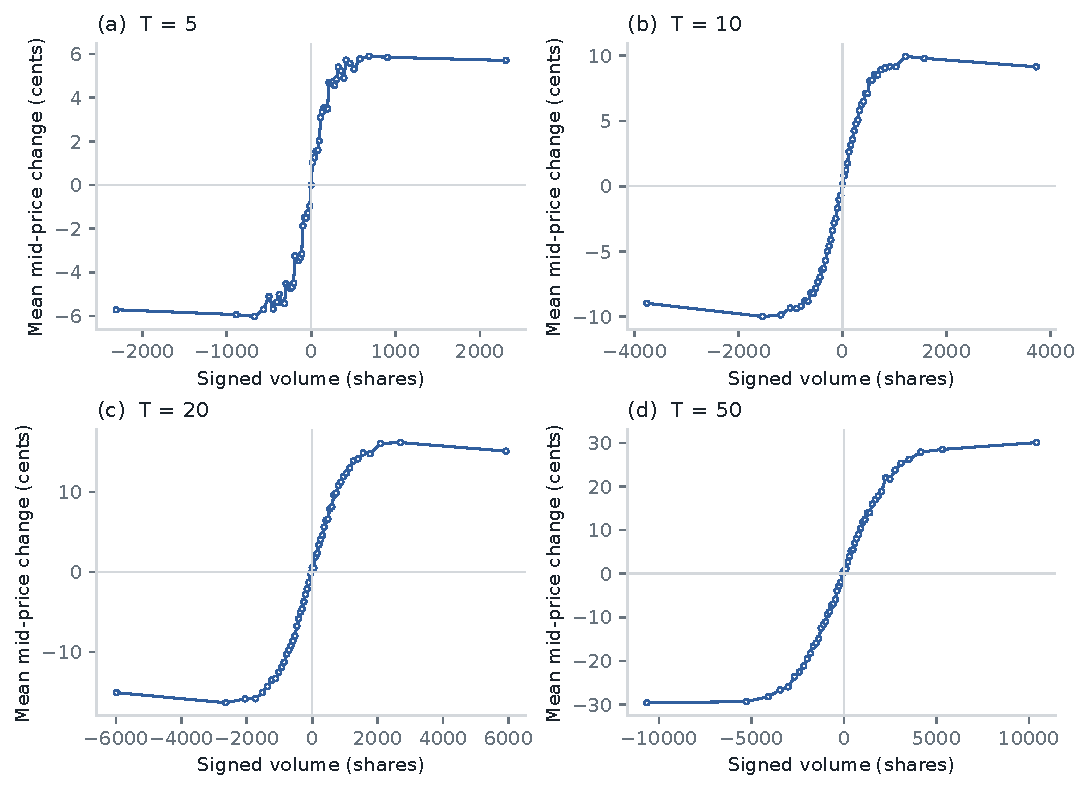
\includegraphics[width=0.78\textwidth]{figures/aggregate-impact.pdf}
  \caption{Mean mid-price change conditional on signed volume. Each point is a
  mean within one of 51 signed-volume quantiles. All \Sessions{} dates enter;
  the bins are not used for model fitting.}
  \label{fig:aggregate}
\end{figure}

A local Kyle slope is also estimated within the central 35 percent of absolute
signed volume. At $T=10$, the fitted value is \KyleLambdaTen{} cents per share.
Across $T\in\{5,10,20,50,100\}$, the fitted slopes decay approximately as
$T^{-\KyleDecay}$. This is a descriptive liquidity estimate, not a trade-level
execution-cost model.

\section{Evaluation design}

\subsection{Chronological holdout}

The main $T=10$ sample contains \TenOrderWindows{} windows across \Sessions{}
dates. The first 80 percent of distinct dates form the training partition; the
remaining dates are held out. Table~\ref{tab:split} gives the exact boundary.
No row is removed from either side of the split.

\begin{table}[H]
  \centering
  \caption{Primary chronological partition.}
  \label{tab:split}
  \begin{tabular}{lll r}
    \toprule
    Partition & First date & Last date & Windows \\
    \midrule
    Train & \TrainFirstDate{} & \TrainLastDate{} & \TrainObservations{} \\
    Holdout & \TestFirstDate{} & \TestLastDate{} & \TestObservations{} \\
    \bottomrule
  \end{tabular}
\end{table}

The four nested OLS specifications are:
\begin{align*}
  \mathcal{M}_1 &: \Delta V, \\
  \mathcal{M}_2 &: \Delta V, |\Delta V|,
    \operatorname{sgn}(\Delta V)\sqrt{|\Delta V|},
    \operatorname{sgn}(\Delta V)\log(1+|\Delta V|), \\
  \mathcal{M}_3 &: \mathcal{M}_2, \Delta E, \\
  \mathcal{M}_4 &: \mathcal{M}_3, |\Delta E|,
    \operatorname{sgn}(\Delta E)\sqrt{|\Delta E|}.
\end{align*}
The transforms are fixed before estimation. An intercept is included. Ridge
regression with standardized $\mathcal{M}_4$ features is retained as a numerical
check, but its predictions are indistinguishable from OLS at the shown
precision.

Scores are calculated only on the holdout:
\begin{align}
  \operatorname{MSE} &= \frac{1}{n}\sum_{i=1}^{n}(y_i-\hat y_i)^2, \\
  R^2 &= 1-\frac{\sum_i(y_i-\hat y_i)^2}
                   {\sum_i(y_i-\bar y)^2}.
\end{align}
Mean absolute error and sign accuracy are reported as secondary diagnostics.
Sign accuracy omits a window when either the realized or fitted response is
exactly zero.

\subsection{Uncertainty and stability checks}

Event-time windows from one session share market conditions. Treating all
windows as independent would understate uncertainty. The bootstrap therefore
resamples the \BootstrapClusters{} complete holdout dates with replacement. For
each of \BootstrapReplicates{} repetitions, scores are recomputed from the
selected daily blocks. The interval is the 2.5th to 97.5th percentile of the
bootstrap distribution.

Five additional temporal splits begin with 40 percent of the dates for
training. Each subsequent block is tested once, then added to the expanding
training set. Horizon checks repeat the 80/20 split for $T=5,10,20,50,100$.
Finally, the response is replaced by
$10{,}000\log(m_{t+T}/m_t)$ to check that the result is not an artifact of
measuring a changing stock price in cents.

\section{Holdout results}

\subsection{Feature ablation}

Table~\ref{tab:models} separates curvature from count information. The linear
volume baseline has \Rtwo{} = \BaselineRtwo{}. Fixed volume transforms account
for the first increase, to \VolumeRtwo{}. Adding only raw signed count reaches
\RawCountRtwo{}. The two additional count transforms change the third decimal
place by less than one point. Raw signed count accounts for the useful part of
the second increase.

\begin{table}[H]
  \centering
  \caption{Full chronological holdout, $T=10$. Errors are measured in cents.}
  \label{tab:models}
  \begin{tabular}{lrrrr}
    \toprule
    Specification & \Rtwo{} & MSE & MAE & Sign accuracy \\
    \midrule
    Signed volume & 0.118 & 147.23 & 8.64 & 77.0\% \\
    Volume transforms & 0.298 & 117.18 & 7.79 & 76.9\% \\
    Volume transforms plus raw signed count & 0.359 & 106.96 & 7.48 & 78.5\% \\
    Volume and count transforms & 0.360 & 106.89 & 7.47 & 78.5\% \\
    \bottomrule
  \end{tabular}
\end{table}

Figure~\ref{fig:calibration} compares fitted and realized means in 20 holdout
bins. The linear volume model spans too narrow a range for the S-shaped response.
The count model follows the binned means more closely, although individual
windows remain noisy.

\begin{figure}[H]
  \centering
  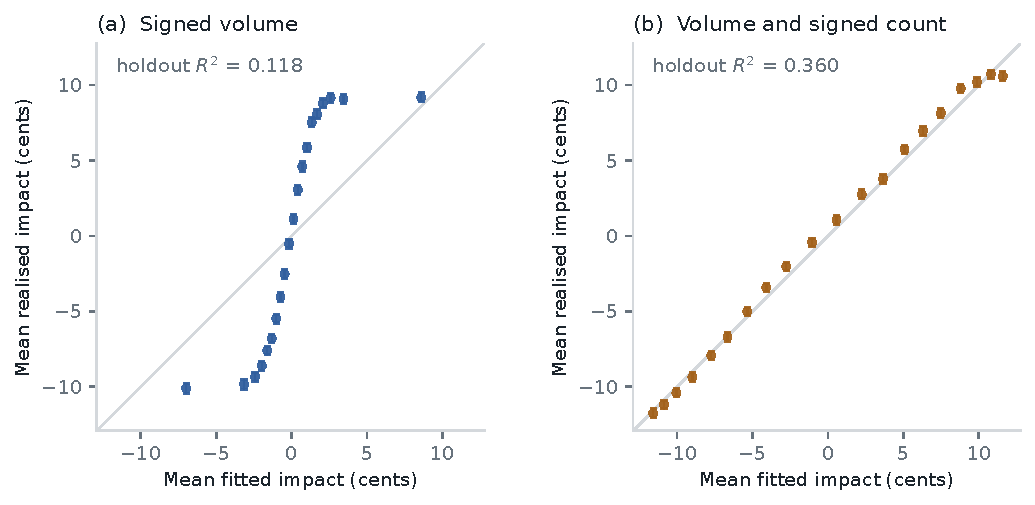
\includegraphics[width=\textwidth]{figures/holdout-calibration.pdf}
  \caption{Holdout calibration by fitted-value quantile. Points show mean fitted
  and realized impact in 20 equally populated bins. Error bars are 1.96
  observation-level standard errors and are included only as a visual guide;
  the formal score interval is clustered by date.}
  \label{fig:calibration}
\end{figure}

Figure~\ref{fig:countresidual} groups the holdout residual of the volume model by
signed count. The mean moves from roughly $-4$ cents for ten sells to more than
3 cents for strong buy counts. This monotone residual pattern is the signal
captured by $\Delta E$.

\begin{figure}[H]
  \centering
  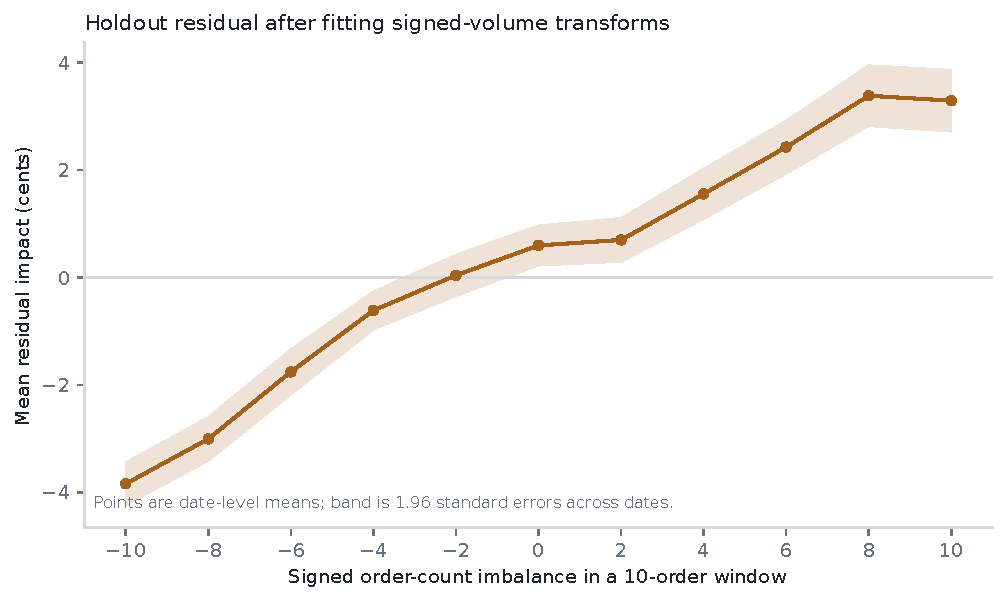
\includegraphics[width=0.75\textwidth]{figures/count-residuals.pdf}
  \caption{Holdout residual from the volume-transform model, grouped by signed
  order count. Points are equal-weighted means across dates. The band is 1.96
  standard errors of the date-level means.}
  \label{fig:countresidual}
\end{figure}

The augmented model lowers MSE from \BaselineMse{} to \AugmentedMse{} cents
squared, a relative reduction of \MseReduction{}. The day-clustered 95 percent
interval is [\BootstrapMseLower{}, \BootstrapMseUpper{}]. The corresponding
increase in \Rtwo{} is \DeltaRtwo{}, with interval
[\BootstrapDeltaLower{}, \BootstrapDeltaUpper{}]. None of the 10,000 bootstrap
draws gives a non-positive improvement. This interval quantifies sampling
variation across the 51 late-year dates. It does not cover model-selection or
cross-year uncertainty.

\subsection{Time and horizon checks}

The count specification outperforms signed volume in every expanding test
block in Figure~\ref{fig:walk}. Its \Rtwo{} ranges from about 0.33 to 0.38, while
the baseline ranges from about 0.10 to 0.14. The gap is present before the final
December block.

\begin{figure}[H]
  \centering
  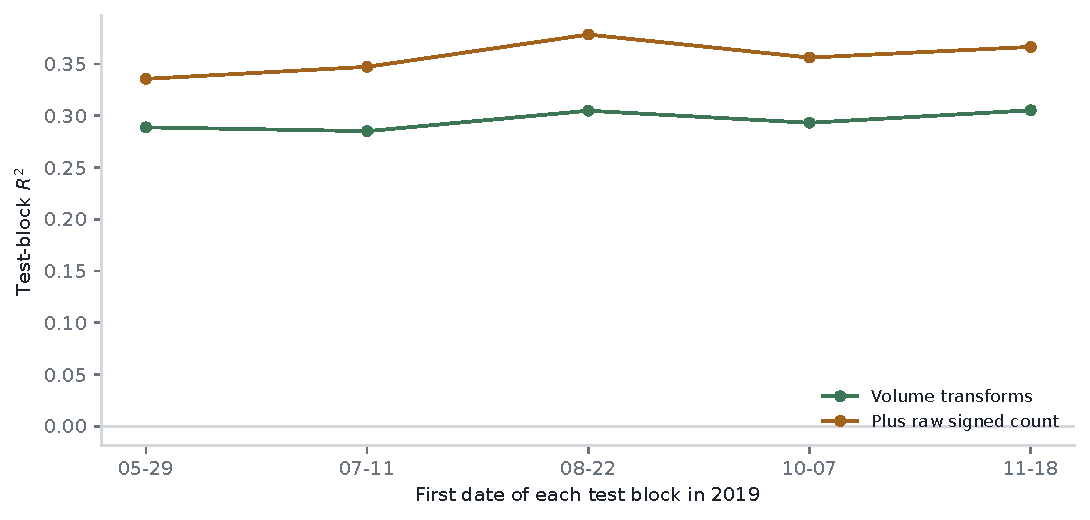
\includegraphics[width=0.92\textwidth]{figures/walk-forward.pdf}
  \caption{Five expanding-window evaluations. Each point is scored on the
  contiguous block beginning at the date shown. Earlier test blocks are added
  to the training set before the next fit.}
  \label{fig:walk}
\end{figure}

The same ordering holds from 5 to 100 orders (Figure~\ref{fig:horizons}). At
$T=5$, \Rtwo{} rises from 0.074 to 0.282. At $T=100$, it rises from 0.269 to
0.482. Longer windows average more idiosyncratic trade-level noise and contain a
wider count range, so higher scores at larger $T$ should not be read as better
short-horizon forecasts.

\begin{figure}[H]
  \centering
  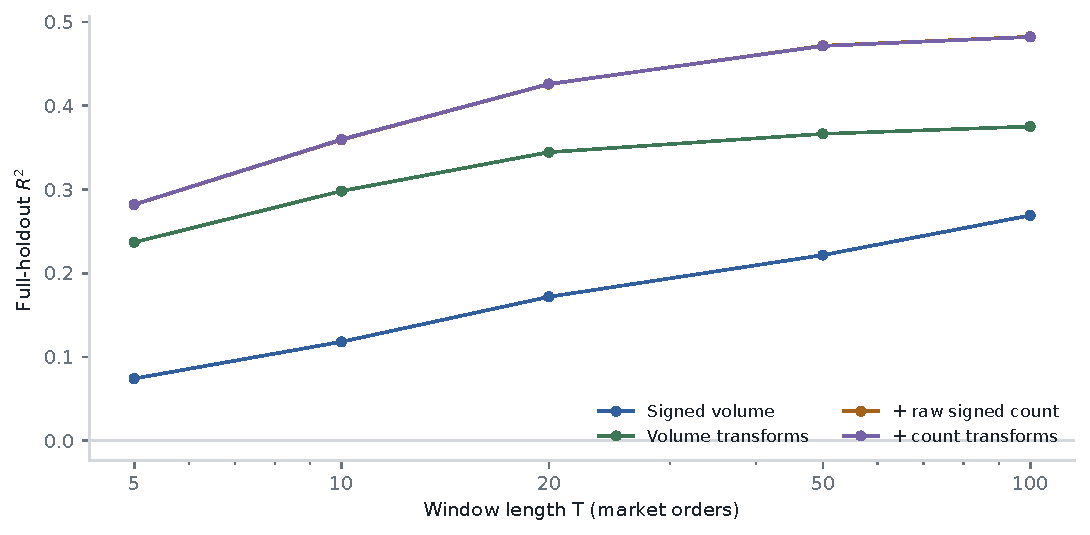
\includegraphics[width=\textwidth]{figures/horizon-robustness.pdf}
  \caption{Full-holdout \Rtwo{} across event-time horizons. The raw count term
  accounts for nearly all of the gap between the volume-transform and full
  specifications.}
  \label{fig:horizons}
\end{figure}

The holdout result is also present within each calendar month. The augmented
\Rtwo{} is 0.329 in the October portion, 0.378 in November, and 0.363 in
December. With log return in basis points as the response, the scores are
\BpsBaselineRtwo{} and \BpsAugmentedRtwo{}, and MSE falls by \BpsMseReduction{}.
Price normalization reduces the size of the gain but does not remove it.

\subsection{Why the previous score was 0.24 to 0.38}

The earlier course protocol removed observations beyond three standard
deviations in both signed volume and realized impact. Re-estimating those bounds
on training dates avoids using the test distribution to set the cutoff, but
applying the impact cutoff to the test still selects observations by the
realized response. Under that trimmed comparison, the baseline has \Rtwo{} =
\TrimmedBaselineRtwo{} and the augmented model has \Rtwo{} =
\TrimmedAugmentedRtwo{}. MSE falls by \TrimmedMseReduction{}.

The trimmed scores describe the retained central sample. Selection on realized
test impact makes them unsuitable as the primary evaluation. The cutoff raises
the baseline much more than the count model, explaining the difference between
0.24 to 0.38 and the untrimmed 0.12 to 0.36 comparison.

\section{Scaling replication}
\label{sec:scaling}

\subsection{Construction}

The scaling exercise follows the aggregate-volume form in
\citet{patzelt2018}. For a window of $N$ timestamp-aggregated type-4 and type-5
transactions, let $Q$ be signed share volume after a daily-volume adjustment,
and let $r$ be the log mid-price change. Conditional curves are estimated in 31
quantile bins for 28 log-spaced horizons from 10 to 5,000 transactions.

Each curve is modeled as
\begin{align}
  \mathcal{R}_N(Q) &= R_N F(Q/Q_N), \\
  F(x) &= \frac{x}{(1+|x|^\alpha)^{\beta/\alpha}}.
\end{align}
One width $Q_N$ and height $R_N$ are estimated per horizon, with a common
$\alpha$ and $\beta$. The nonlinear fit uses observation-count weights and a
soft-L1 loss. Figure~\ref{fig:collapse} plots the resulting rescaled curves. The
collapse is close over the central observed range, with more dispersion around
the origin and at a few long-horizon curves.

\begin{figure}[tbp]
  \centering
  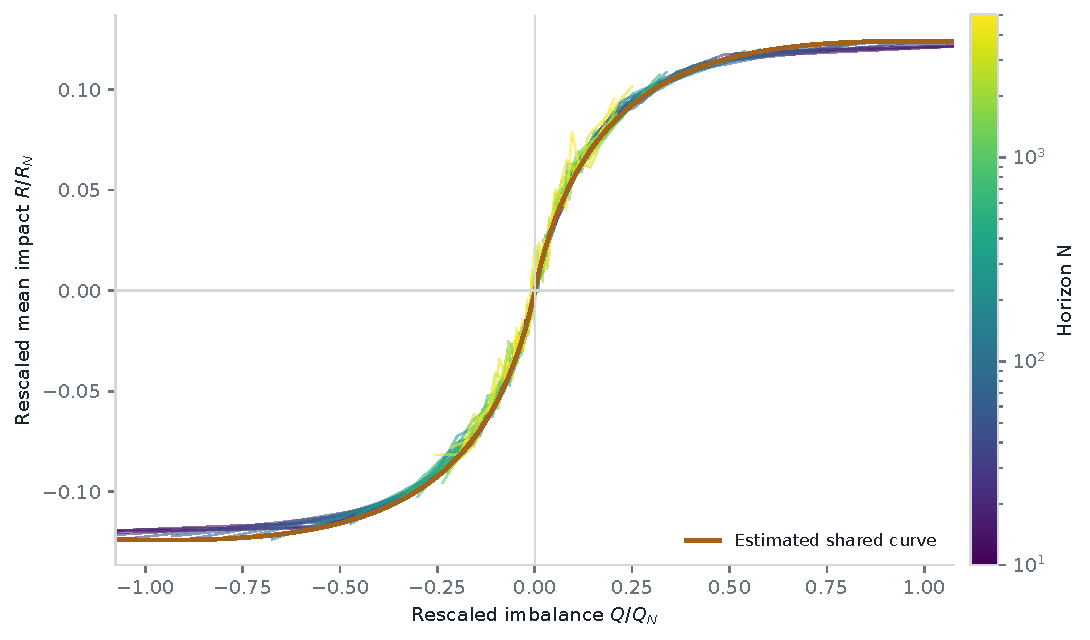
\includegraphics[width=0.82\textwidth]{figures/scaling-collapse.pdf}
  \caption{Finite-size scaling collapse for TSLA 2019. Color identifies the
  aggregation horizon. The orange line is the common fitted shape. This is an
  in-sample curve construction, not a forecast evaluation.}
  \label{fig:collapse}
\end{figure}

\subsection{Scale fits and interpretation}

After the curve fit, the scale parameters are regressed on horizon in log space:
\begin{equation}
  Q_N = a_Q N^{\xi}, \qquad R_N = a_R N^{\psi}.
\end{equation}
Table~\ref{tab:scales} and Figure~\ref{fig:scales} report those second-stage
fits. The width exponent is \WidthExponent{} and the height exponent is
\HeightExponent{}. The residual panels show that the largest horizons carry the
main deviations from a straight power law.

\begin{table}[H]
  \centering
  \caption{Log-log fits to the 28 estimated scale parameters. Standard errors
  condition on the first-stage scale estimates.}
  \label{tab:scales}
  \begin{tabular}{lrrr}
    \toprule
    Scale & Exponent & Standard error & In-sample \Rtwo{} \\
    \midrule
    Width $Q_N$ & \WidthExponent{} & \WidthExponentSe{} & \WidthFitRtwo{} \\
    Height $R_N$ & \HeightExponent{} & \HeightExponentSe{} & \HeightFitRtwo{} \\
    \bottomrule
  \end{tabular}
\end{table}

\begin{figure}[tbp]
  \centering
  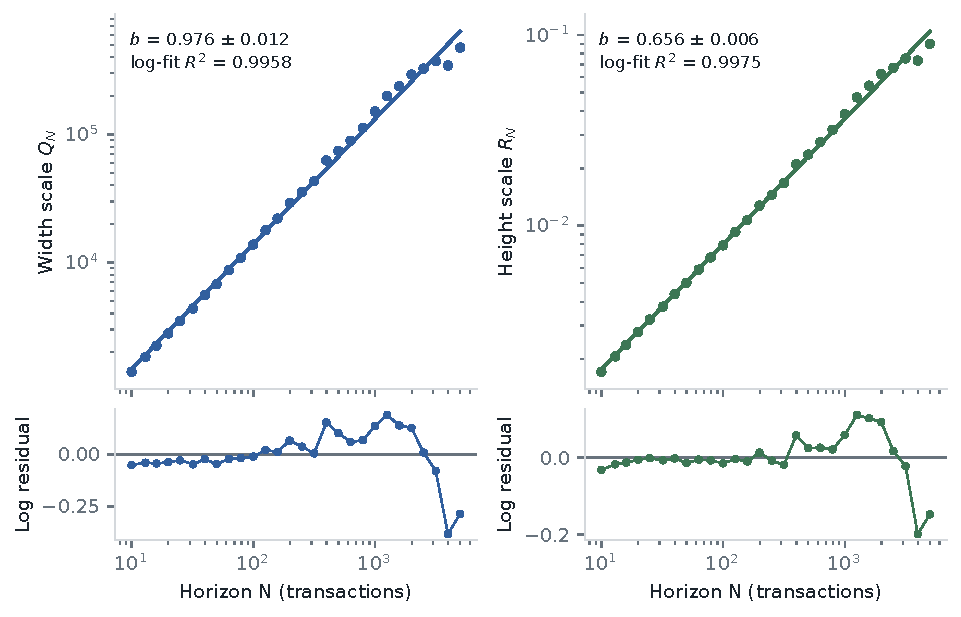
\includegraphics[width=\textwidth]{figures/scaling-fits.pdf}
  \caption{Power-law fits for the estimated width and height scales. Lower
  panels show log residuals. The displayed \Rtwo{} values describe these 28
  in-sample points only.}
  \label{fig:scales}
\end{figure}

Near zero imbalance, the master-curve slope scales as $R_N/Q_N$. The fitted
exponents imply a decay $N^{-(\xi-\psi)}$ with
$\xi-\psi=\ScaleSlopeDecay{}$. The local Kyle slopes in
Section~\ref{sec:measurement} decay with exponent \KyleDecay{}. The two
calculations use different transaction samples and return definitions, so their
agreement is descriptive.

The order-sign standard deviation gives a Hurst exponent of \SignHurst{}, in
line with persistent trade signs in this sample. The \WidthFitRtwo{} and
\HeightFitRtwo{} values belong to regressions on 28 estimated scale points.
They do not measure future price variation. This dataset supports a replication
of the proposed scaling form on TSLA 2019; the cross-asset claim in
\citet{patzelt2018} requires a broader panel.

\section{Limitations}

\begin{itemize}
  \item The variables and response cover the same window, and order flow is
  endogenous. The fitted coefficients are neither pre-trade forecasts nor
  causal price effects.
  \item Timestamp and side grouping cannot recover investor identity or
  institutional metaorders. The book covers NASDAQ rather than consolidated US
  liquidity, and hidden-execution signs are uncertain around the midpoint.
  \item The feature family grew out of the course analysis. Although dates are
  held out chronologically, there is no second untouched year after the feature
  comparison. The bootstrap does not account for that research process.
  \item The scaling standard errors treat first-stage $Q_N$ and $R_N$ estimates
  as data. They do not propagate all curve-fitting uncertainty, and overlapping
  information across horizons remains.
  \item TSLA in 2019 is one liquidity regime. Neither the count result nor the
  fitted exponents can be assumed to hold for another asset or year.
\end{itemize}

\section{Reproducibility and provenance}

The Python package reconstructs the two transaction tables, builds event-time
windows, fits the models, and writes the aggregate files under
\texttt{results/}. The figures are vector PDFs. Synthetic tests cover file
pairing, book alignment, day boundaries, chronological splits, clustered
resampling, and the scaling regressions. Reproducing the annual tables requires
licensed LOBSTER files, which are not tracked.

The course presentation lists L. Cohen, R. Darwish, A. Pariente, H. Rohrbach,
and R. Sithisak. Anastasia Bugaenko supervised the work. I wrote this standalone
package and report after the group project; the collaborative repository remains
separate.

\section{Conclusion}
\vspace{0.2em}

On the complete late-2019 holdout, adding signed count to the volume model moves
\Rtwo{} from \BaselineRtwo{} to \AugmentedRtwo{} and reduces MSE by
\MseReduction{}. Raw count accounts for almost all of that gain. The ordering is
stable across the time and horizon checks reported above.

TSLA's 2019 conditional curves also fit the scaling form proposed by
\citet{patzelt2018}. That is a replication on one stock-year. The supervised
model is evaluated by the chronological score.

\bibliographystyle{plainnat}
\bibliography{references}

\end{document}
